\documentclass[twoside,twocolumn]{article}

\usepackage{blindtext} 
\usepackage{graphicx}
\usepackage[sc]{mathpazo} 
\usepackage[T1]{fontenc} 
\linespread{1.05} 
\usepackage{microtype} 

\usepackage[utf8]{inputenc} 


\usepackage[spanish,english]{babel} 



\usepackage[hmarginratio=1:1,top=32mm,columnsep=20pt]{geometry} 
\usepackage[hang, small,labelfont=bf,up,textfont=it,up]{caption} 
\usepackage{booktabs} 


\usepackage{lettrine} 


\usepackage{enumitem} 
\setlist[itemize]{noitemsep} 


\usepackage{abstract} 
\renewcommand{\abstractnamefont}{\normalfont\bfseries} 
\renewcommand{\abstracttextfont}{\normalfont\small\itshape} 


\usepackage{titlesec} 
\renewcommand\thesection{\Roman{section}} % 
\renewcommand\thesubsection{\roman{subsection}} 
\titleformat{\section}[block]{\large\scshape\centering}{\thesection.}{1em}{} 
\titleformat{\subsection}[block]{\large}{\thesubsection.}{1em}{} 


\usepackage{fancyhdr} 
\pagestyle{fancy} 
\fancyhead{} 
\fancyfoot{} 
\fancyhead[C]{Patrones de Diseño $\bullet$ Octubre 2020 $\bullet$ } 
\fancyfoot[RO,LE]{\thepage} 


\usepackage{titling} 


\usepackage{hyperref} 


%----------------------------------------------------------------------------------------
%	TILULOS
%----------------------------------------------------------------------------------------


\setlength{\droptitle}{-4\baselineskip} 

\pretitle{\begin{center}\Huge\bfseries} 
\posttitle{\end{center}} 
\title{Patrones de Diseño} 
\author{Percy Taquila Carazas}
\date{\today} 
\renewcommand{\maketitlehookd}{

\selectlanguage{english}
\begin{abstract}
\noindent 
Aca va el asbtract(ingles)
\end{abstract}


\selectlanguage{spanish}
\begin{abstract}
\noindent 
Aca va el resumen
\end{abstract}

}

%----------------------------------------------------------------------------------------

\begin{document}

% Print the title
\maketitle

%----------------------------------------------------------------------------------------
%	INTRODUCCION
%----------------------------------------------------------------------------------------

\section{Introduccion}

\lettrine[nindent=0em,lines=3]{E}l aprendizaje es esencial para la mayoría de las arquitecturas de redes neuronales, por lo que la elección de un algoritmo de aprendizaje es un punto central en el desarrollo de una red, este implica que una unidad de procesamiento es capaz de cambiar su comportamiento entrada/salida
como resultado de los cambios en el medio.\\

El camino hacia la construccion de maquinas inteligentes comienza en la Segunda Guerra Mundial con el diseÑo de computadoras analogicas ideadas para controlar cañones antiaereos o para la navegacion.
Algunos investigadores observaron que existıan semejanzas entre el funcionamiento de estos dispositivos de control y los sistemas reguladores de los seres vivos. De este modo, combinando los avances de la electronica de la posguerra y los conocimientos sobre los sistemas nerviosos de los seres vivos, inicio el reto de construir maquinas capaces de responder y aprender como los animales.




%----------------------------------------------------------------------------------------
%	Objetivos
%----------------------------------------------------------------------------------------


\section{Desarrollo}
En el aprendizaje supervisado debemos aprender a entrenar a la neurona, haciendo uso de ecuaciones matemáticas, para balancear sus pesos

A diferencia del aprendizaje supervisado, en el no supervisado solo se le otorgan las características, sin proporcionarle al algoritmo ninguna etiqueta. Su función es la agrupación, por lo que el algoritmo debería catalogar por similitud y poder crear grupos, sin tener la capacidad de definir cómo es cada individualidad de cada uno de los integrantes del grupo.



%----------------------------------------------------------------------------------------
%	Conclusiones
%----------------------------------------------------------------------------------------


\section{Conclusiones}

El Aprendizaje Automatizado (Machine Learning; ML) es una rama de la inteligencia artificial, en gran parte inspirada en el razonamiento humano, que comprende el aprendizaje a partir de experiencia (Sammut y Webb 2011)(Sammut y Webb 2011). El aprendizaje automático aborda, a su vez, una serie de problemáticas que tributan a problemas específicos, entre ellos: los problemas de clasificación, asociación, agrupamiento, y selección de rasgos (Sammut y Webb 2011)(Cong, Pérez y Morell 2015; Sammut y Webb 2011).
Mediante el aprendizaje automático, el reconocimiento de patrones, va aprendiendo y mejora conforme a la experiencia que va adquiriendo. Para lograr su aprendizaje lo hace mediante dos formas: uno es el aprendizaje supervisado, o también llamado clasificación, y el otro es el aprendizaje no supervisado o agrupamiento.

%----------------------------------------------------------------------------------------
%	Recomendaciones
%----------------------------------------------------------------------------------------

\section{Recomendaciones}


\begin{itemize}
\item Aprendizaje Supervisado
En el Aprendizaje Supervisado los datos para el entrenamiento incluyen la solución deseada, llamada «etiquetas» (labels). Un claro ejemplo es al clasificar correo entrante entre Spam o no. Entre las diversas características que queremos entrenar deberemos incluir si es correo basura o no con un 1 o un 0. Otro ejemplo son al predecir valores numéricos por ejemplo precio de vivienda a partir de sus características (metros cuadrados, nº de habitaciones, incluye calefacción, distancia del centro, etc.) y deberemos incluir el precio que averiguamos en nuestro set de datos.

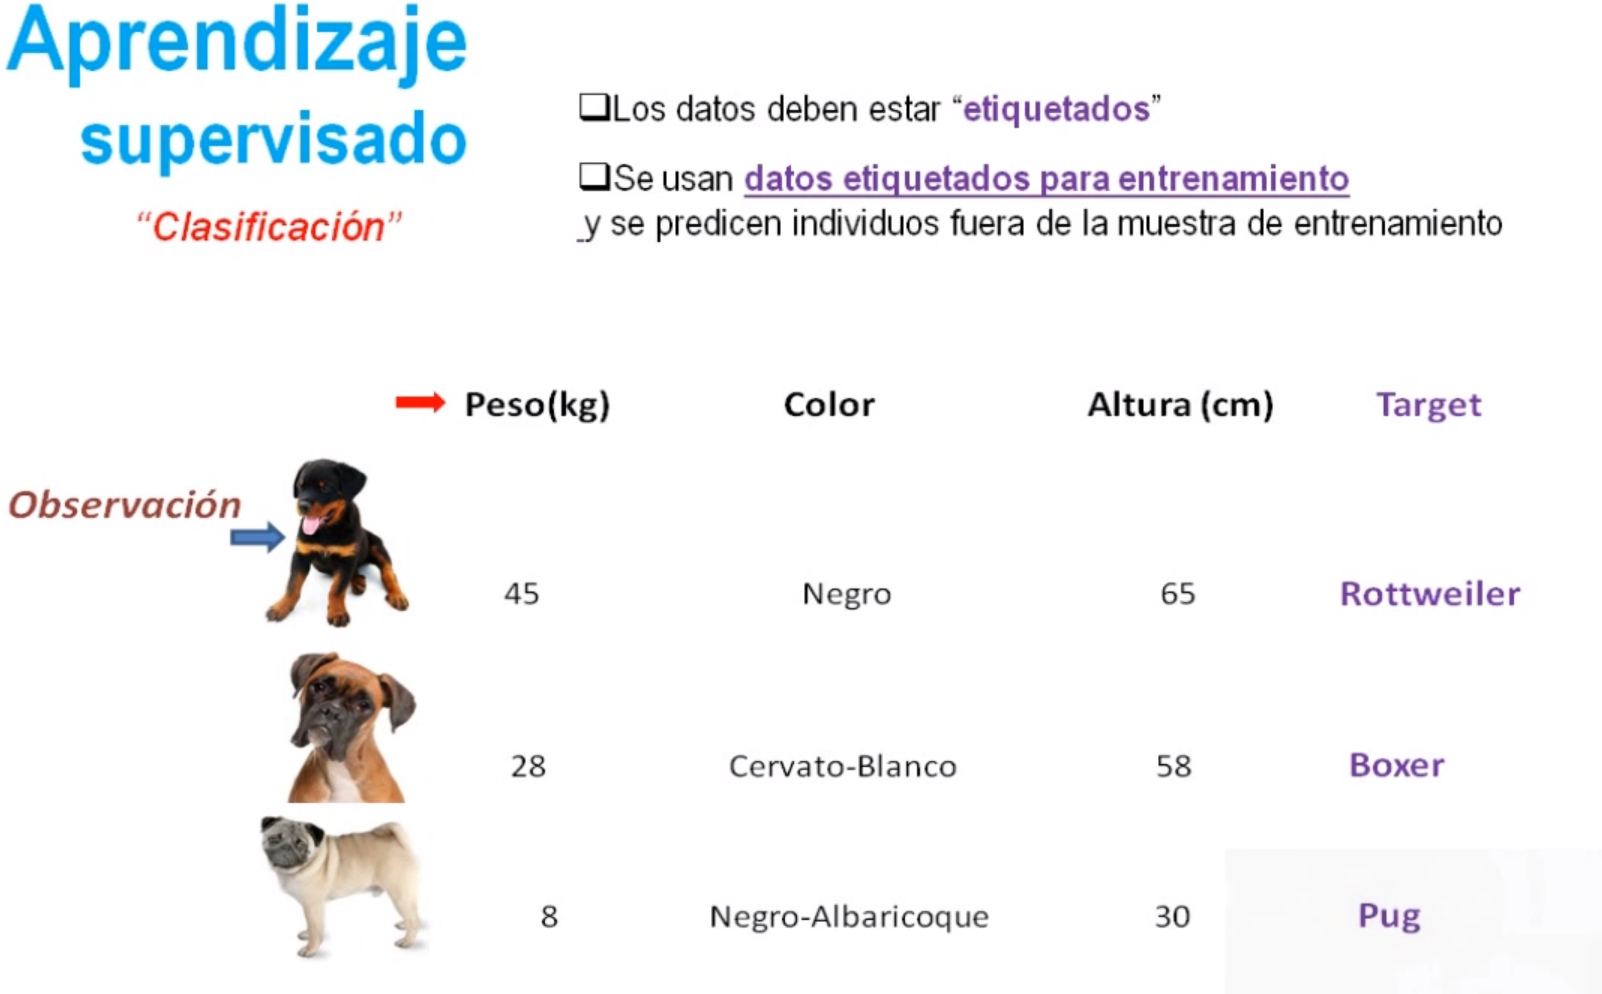
\includegraphics[width=7cm]{Imagenes/imagen1}

\end{itemize}



%----------------------------------------------------------------------------------------
%	BIBLIOGRAFIA
%----------------------------------------------------------------------------------------

\selectlanguage{spanish}
\begin{thebibliography}{99} 

\bibitem[1]{}
\newblock Javier Lozado Silva, 2018. Aprendizaje Supervisado Eficiente
Para el analisis de datos 
 



\end{thebibliography}


%----------------------------------------------------------------------------------------


\end{document}
